\section{Transformer Models}\label{TM}
Transformer models have become the foundation of modern \ac{NLP} due to their ability to capture complex relationships between words — even when those words are far apart in a sentence.
Unlike older models such as \ac{RNN}, which process text sequentially and struggle with long-range dependencies, Transformers process entire sequences in parallel.
Their core innovation is the \textbf{self-attention} mechanism, which allows the model to weigh the relevance of each word with respect to others in the sequence.

A Transformer is a deep neural network architecture introduced by Vaswani et al.~\cite{vaswani_attention_2023}.
It has since become the basis of widely-used models such as BERT and GPT, which are trained on large corpora in a self-supervised manner, that is, without labeled data.

Transformers are primarily composed of an encoder and a decoder block, as illustrated in Figure~\ref{fig:encoderDecoder}.
The encoder processes the input sequence and generates contextual representations.
The decoder then uses these representations, along with previously generated tokens, to produce the output sequence.
This architecture enables applications such as machine translation, summarization, and text generation.


%This indicates that the model is optimize to develop an understanding of its inputs. 
%The decoder creates a target sequence using the encoder's representation (features) and other inputs. 
%This indicates that the model is optimized to generate an output. 

\begin{figure}[htb]
    \centering
    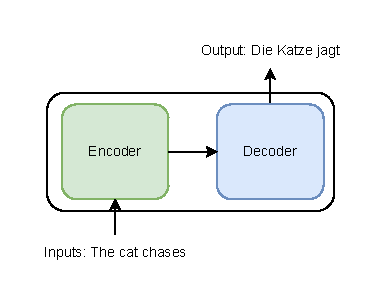
\includegraphics[width=0.45\linewidth]{Abschlussarbeit/Pictures/encoder_decoder_simple (1).pdf}
    \caption{Encoder-decoder structure of a Transformer.}
    \label{fig:encoderDecoder}
\end{figure}

A key strength of Transformer models is their self-attention mechanism, which enables them to weigh different parts of the input when making predictions.

For example, in the sentence:
\textit{``The cat chased the mouse because she was hungry.''
}
a Transformer can learn that ``she`` refers to ``the cat`` by attending to all words in the sequence at once.

%There are different models that are based on transformer. 

%\textbf{{BERT}} \cite{BERT} is an encoder model and uses only the encoder of a Transformer model. 
%BERT stands for \textbf{B}idirectional \textbf{E}ncoder \textbf{R}epresentations from \textbf{T}ransformers.
%BERT is designed to pre-train deep bidirectional representations from unlabeled text.
%Unlike recent language representation models \cite{peters-etal-2018-deep, GPT}, BERTS attention layer can access all words in the initial sentence in each step.
%Therefore, the pre-trained BERT model can be optimized without significant task-specific architectural changes with just one more output layer to create state-of-the-art models for a variety of tasks, including language inference and question answering.
%Models like that are often characterized as having a bi-directional attention and are called auto-encoding models.
%For tasks that require an understanding of the whole sentence, such as sentence classification, named entity recognition and extractive question answering are encoder models best suited.

%\textbf{GPT} \cite{GPT} is a decoder model and only uses the decoder of a Transformer model and a shortcut for Generative Pre-Training.
%GPT is a semi-supervised approach to language understanding tasks and is trained through a combination of unsupervised pre-training and supervised fine-tuning. 
%The attention layer can access only the words positioned before a given word in the sentence and are often called auto-regressive models.
%The goal is to learn a universal representation that can be easily adapted to different tasks. The approach involves a two-stage training procedure in which the initial parameters of the neural network model are learned on unlabeled data and adapted to the target tasks.


Two of the most influential Transformer-based language models are \textbf{BERT} and \textbf{GPT}, which differ in their architecture and training objective.

\paragraph{BERT – Bidirectional Encoder Representations from Transformers}
BERT~\cite{BERT} is an \textit{encoder-only} model. It processes the entire input sentence at once using bidirectional self-attention and is designed to learn contextual representations from unlabeled text through a masked language modeling objective.

Unlike earlier models~\cite{peters-etal-2018-deep, GPT}, BERT’s attention layers can access all tokens in the sequence during training. This allows it to capture both left and right context simultaneously. Models of this type are referred to as \textit{auto-encoding models}.
Thanks to its pre-training on large corpora and its architecture, BERT can be fine-tuned with minimal task-specific modifications for a wide range of NLP tasks, including sentence classification, named entity recognition, and extractive question answering.

\paragraph{GPT – Generative Pre-Training}
GPT~\cite{GPT} is a \textit{decoder-only} model. It uses unidirectional (left-to-right) attention and is trained to predict the next word in a sentence, making it well suited for text generation tasks.

GPT follows a two-stage training approach:
\begin{itemize}
    \item \textbf{Unsupervised pre-training} on raw text to learn general-purpose language representations.
    \item \textbf{Supervised fine-tuning} on task-specific labeled data.
\end{itemize}

Because GPT can only attend to preceding tokens at each position, it is called an \textit{auto-regressive model}.

%\paragraph{Summary of Model Types}
%\begin{itemize}
%    \item \textbf{BERT} (encoder-only) $\rightarrow$ for \textit{understanding} text.
%    \item \textbf{GPT} (decoder-only) $\rightarrow$ for \textit{generating} text.
%\end{itemize}

%\vspace{0.5em}
%\noindent

